\documentclass[paper=letter, fontsize=12pt]{scrartcl}
\usepackage[T1]{fontenc}
\usepackage{fourier}
\usepackage[
top=2.5cm,
bottom=2.5cm,
left=2.5cm,
right=2.5cm,
headheight=17pt, 
includehead,includefoot,
heightrounded, 
]{geometry}
\usepackage[spanish,es-tabla]{babel}
\decimalpoint
\usepackage[protrusion=true,expansion=true]{microtype}	
\usepackage{amsmath,amsfonts,amsthm} % Math packages
\usepackage[pdftex]{graphicx}	
\usepackage{url}
\usepackage{epsfig, graphics, graphicx,subfigure, tabularx}
\usepackage{gensymb}
\usepackage{listings}%\addcontentsline{toc}{chapter}{\'Indice de tablas}
\usepackage{multirow}

%%% Custom sectioning
\usepackage{sectsty}
\allsectionsfont{\centering \normalfont\scshape}


%%% Custom headers/footers (fancyhdr package)
\usepackage{fancyhdr}
\pagestyle{fancyplain}
\fancyhead{}											% No page header
\fancyfoot[L]{}											% Empty 
\fancyfoot[C]{}											% Empty
\fancyfoot[R]{\thepage}									% Pagenumbering
\renewcommand{\headrulewidth}{0pt}			% Remove header underlines
\renewcommand{\footrulewidth}{0pt}				% Remove footer underlines
\setlength{\headheight}{13.6pt}


%%% Equation and float numbering
\numberwithin{equation}{section}		% Equationnumbering: section.eq#
\numberwithin{figure}{section}			% Figurenumbering: section.fig#
\numberwithin{table}{section}				% Tablenumbering: section.tab#


%%% Maketitle metadata
\newcommand{\horrule}[1]{\rule{\linewidth}{#1}} 	% Horizontal rule

\title{
	%\vspace{-1in} 	
	\usefont{OT1}{bch}{b}{n}
	
	\horrule{0.5pt} \\[0.4cm]
	\large Estudio te\'orico de propiedades magn\'eticas en [Pt,V] (Se,S)\textsubscript{2} y experimentación de efecto Kerr en CoFeB  \\
	\horrule{2pt} \\[0.2cm]
	\normalfont \normalsize \textsc{Cuarto Avance de Tesis} \\ [5pt]
}
\author{
	\normalfont 								\normalsize
	Gabriel Adona\'i Mart\'inez Zepeda \\[-1pt]		\normalsize
	\today
}
\date{}
\includeonly{IntrRep}
\begin{document}
	\maketitle
	\section{Introducci\'on}
	En el presente reporte se centra  en el desarrollo de un espectr\'ometro por efecto Kerr  magneto-\'optico. La raz\'on para desarrollar esta clase de espectr\'ometro se debe  que es una de las principales t\'ecnicas no invasivas para medir propiedades magn\'eticas de materiales. Este fen\'omeno se basa en  los cambios de la luz reflejada por un material magn\'etico y que se refleja principalmente con los cambios en la polarizaci\'on e intensidad de la luz \cite{MOp-1997}. Este fenómeno es utilizado para obtener la hist\'eresis del material ferromagn\'etico y de la cual se puede medir la anisotrop\'ia magn\'etica y los campos de cohersi\'on, principalmente \cite{MOp-2008}. M\'as a\'un, si el efecto Kerr se mide en funci\'on de la longitud de onda del haz incidente, \'este provee informaci\'on valiosa acerca de los efectos del campo  magn\'etico en la estructura electr\'onica del material \cite{MOp-1997}.
	
	\section{Efecto Kerr magneto-\'optico}
	Una manera de estudiar las propiedades magn\'eticas de los materiales es haciendo uso de los efectos magneto-\'opticos, los cuales surgen como resultado de la interacci\'on entre la luz y la materia que es sujeta a un campo magn\'etico y que en el caso de materiales que tengan cierto orden magn\'etico, tales como los materiales ferromagn\'eticos, se siguen observando estos fen\'omenos en el caso de que no se apliquen campos magn\'eticos externos. Dichos fen\'omenos provienen de la separaci\'on de niveles de energ\'ia inducidos por la aplicaci\'on de un campo magn\'etico externo; es decir proviene del efecto Zeeman y lo cual provoca que cambie el espectro del coeficiente de  absorbci\'on y tiende a la aparici\'on o a la variaci\'on de la anisotropía magn\'etica. La anisotrop\'ia de un medio magnetizado se puede observar en la reflexi\'on de la luz en la superficie, el cual es el llamado efecto Kerr magneto-\'optico, que fue descubierto por  John Kerr en 1888 observando el cambio de polarizaci\'on  lineal a el\'iptica provocado por la reflexi\'on de la luz en un electro im\'an pulido \cite{Kerr_1888}.  En la espectroscopia de efecto Kerr magneto-\'optico generalmente se distingue entre la polarizaci\'on lineal incidente entre $s$ y $p$, en las cuales el campo el\'ectrico est\'a normal ($s$) o paralelo ($p$) al plano de incidencia y estas propiedades magneto-\'opticas dependen de las polarizaciones $s$ y $p$  \cite{mo_2004}. Se pueden caracterizar tres tipos de  efecto Kerr dependiendo de la orientaci\'on del vector de magnetizaci\'on con respecto a la superficie y al plano de incidencia del haz: polar, longitudinal y transversal, los cuales se observan en la figura \ref{Kerr:fig:Conf}. La configuraci\'on polar (fig. \ref{Kerr:fig:pol}) se tiene cuando el vector de magnetizaci\'on se orienta en la direcci\'on perpendicular a la superficie del material y paralelamente al plano de incidencia. La geometr\'ia longitudinal (fig. \ref{Kerr:fig:long}) se obtiene cuando se orienta el vector de magnetizaci\'on paralelamente a la superficie del material y al plano de incidencia y la configuraci\'on transversal se da cuando se orienta perpendicularmente al plano de incidencia y  paralelamente a la superficie.  La influencia de la magnetizaci\'on el las configuraciones polar  y longitudinal provoca la rotaci\'on del plano de polarizaci\'on y la aparici\'on de  la elipticidad de la luz reflejada. En cambio en la configuraci\'on transversal, solo se observa el cambio de la intensidad y la fase del haz incidente \cite{mo_2004}.
	\begin{figure}[!hbt]
		\centering
		\subfigure[polar]{
			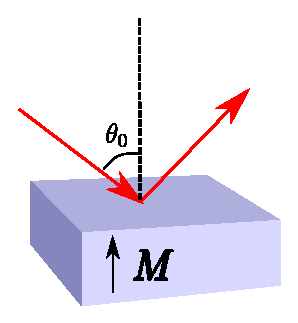
\epsfig{file=figKerr/pol/pol.eps, width=4.0cm,height=4.0cm}
			\label{Kerr:fig:pol}
		}
		\subfigure[longitudinal]{
			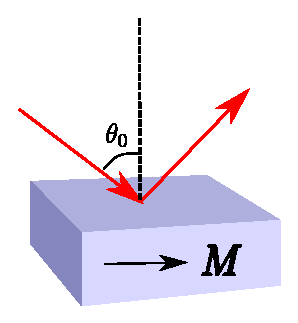
\epsfig{file=figKerr/pol/long.eps, width=4.0cm,height=4.0cm}
			\label{Kerr:fig:long}
		}
		\subfigure[transversal]{
			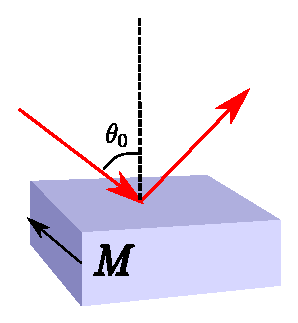
\epsfig{file=figKerr/pol/trans.eps, width=4.0cm,height=4.0cm}
			\label{Kerr:fig:trans}
		}
		\caption[Configuraciones de Efecto Kerr magneto-\'optico.]{Diferentes configuraciones del efecto Kerr magneto-\'optico}
		\label{Kerr:fig:Conf}
	\end{figure}

\section{Montaje experimental}
En la figura \ref{Met:fig:kerr} se muestra el montaje experimental utilizado para medir el efecto Kerr magneto-\'optico en configuraci\'on longitudinal. El sistema est\'a pensado para realizar mediciones variando el campo magn\'etico externo, las cuales son \'utiles para caracterizar las propiedades magn\'eticas del los materiales; es decir funcionar\'ia como un magnet\'ometro y se puede variar la longitud de onda lo cual es de gran utilidad para caracterizar los cambios en las propiedades electr\'onicas de los materiales bajo la influencia de un campo magn\'etico externo.
\begin{figure}[!hbt]
	\centering
	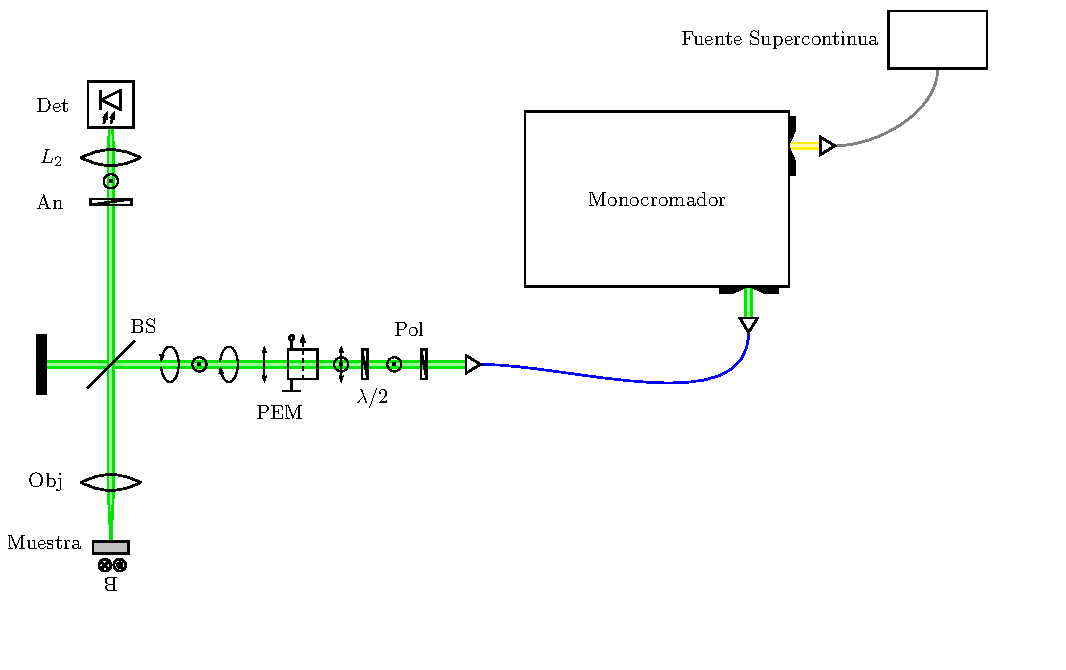
\includegraphics[scale=0.6]{figMet/diagrama/diagrama.pdf}
	\caption[Montaje experimental de espectroscop\'ia de efecto kerr magneto-\'optico.]{Montaje experimental para medir el efecto Kerr Mageto-\'optico en configuraci\'on longitudinal. La fiente supercontinua abarca un espectro de $430~nm $ a $2400~nm$ nm con una frecuencia de repetici\'on que var\'ia de $10~kHz $ a $80~MHz$ }
	\label{Met:fig:kerr}
\end{figure}
\subsection{Procesado de la informaci\'on}
Se utiliz\'o el an\'alisis de matrices de Jones \cite{fuji_2005} para deducir una expresi\'on de la intensidad de la luz que llega al detector y  se obtiene un par de expresiones para las razones de la intensidad que detecta el lock in cuando se encuentra sincronizado con el primer y segundo arm\'onico del retardo del modulador fotoel\'astico:
\begin{eqnarray}
	I_{1f}/I_{dc} &=& 4 J_1 (\Psi_0) ~\tan(\varPsi) ~(\theta_k ~\sin(\Delta) - \eta_k~ \cos(\Delta)) \label{Met:ec:divI1}\\
	I_{2f}/I_{dc} &=& -4 J_2 (\Psi_0) ~\tan(\varPsi) ~(\theta_k~\cos(\Delta) + \eta_k ~ \sin(\Delta)) \label{Met:ec:divI2}.
\end{eqnarray}
En este caso $I_0$ es detectada por el mult\'imetro digital. Se utiliza un programa desarrollado en LabVIEW, el cual es utilizado para controlar el monocromador  y el PEM as\'i como para adquirir informaci\'on del amplificador lock in y del mult\'imetro. Una vez que se tienen estos valores se realiza la raz\'on entre el valor del lock in y el del mult\'imetro de tal forma que se obtienen las expresiones \ref{Met:ec:divI1} y \ref{Met:ec:divI2} dependiendo de que si el lock in est\'a sincronizado a $f$ o $2f$.  Este programa le permite al usuario realizar mediciones variando la longitud de onda o medir el ciclo de hist\'eresis variando el campo magn\'etico externo aplicado a la muestra.
\newline
\par De acuerdo con las ecuaciones \ref{Met:ec:divI1} y \ref{Met:ec:divI2} se observa que es necesario realizar un an\'alisis mas detallado debido a que no es posible obtener los valores  para la rotaci\'on ($\theta_k$) y la elipticidad ($\varepsilon_k$) Kerr de forma directa, dado  que en estas expresiones aparecen mezcladas en ambas ecuaciones. Es posible encontrar los valores para la rotaci\'on  y la elipticidad si se tratan las expresiones \ref{Met:ec:divI1} y \ref{Met:ec:divI2} como un sistema de ecuaciones, para lo cual es necesario conocer los valores de $\varPsi (eV)$ y $\Delta (eV)$ del beamsplitter. Estos valores fueron posible conocerlos realizando una medici\'on de elipsometr\'ia a $70\degree$ cuyos valores se observan en la figura \ref{Met:fig:ElipBS} junto con su ajuste realizado con el programa WVASE. 
\begin{figure}[!hbt]
	\centering
	\subfigure[valores de $\Psi$]{
		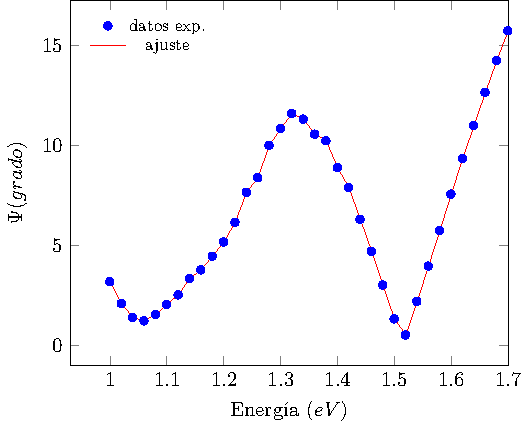
\includegraphics[scale=0.75]{figMet/figElips/grafPsi}
		\label{Met:fig:PsiBS}
	}
	\subfigure[valores de $\Delta$]{
		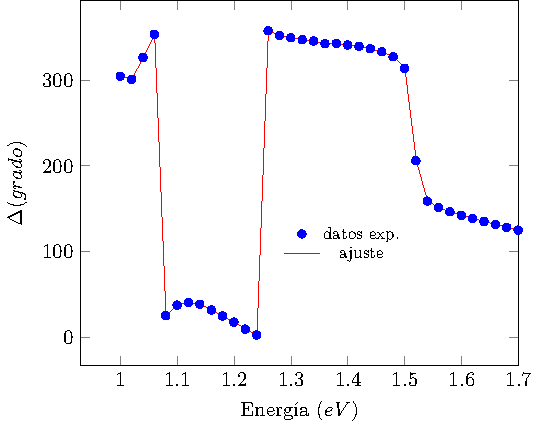
\includegraphics[scale=0.75]{figMet/figElips/grafTheta}
		\label{Met:fig:DeltaBS}
	}
	\caption[Gr\'aficas de $\Psi$ y $\Delta$ del beamspliter a $70 \degree$.]{valores experimentales a $70\degree$  para $\Psi$ y $\Delta$ del beamsplitter en funci\'on de la energ\'ia del fot\'on con su ajuste.} 
	\label{Met:fig:ElipBS}
\end{figure}
\par En base con este ajuste es posible estimar los valores de $\varPsi (eV)$ y $\Delta (eV)$ para $45 \degree$ con ayuda de WVASE que se muestran en la figura \ref{Met:fig:ElipBS45}. Como se puede observar estos dos par\'ametros presentan grandes variaciones en todo el espectro  por lo que fue necesario implementar una rutina en Python  para poder obtener  los valores de la elipticidad  y el \'angulo Kerr resolviendo el sistema de ecuaciones (\ref{Met:ec:divI1} y \ref{Met:ec:divI2}).
\begin{figure}[!hbt]
	\centering
	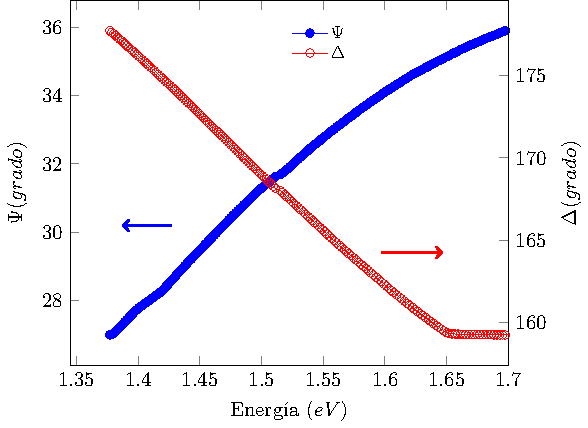
\includegraphics[scale=1.1]{figMet/figElips/grafPsidelta45.pdf}
	\caption[Gr\'aficas de $\Psi$ y $\Delta$ del beamspliter a $70 \degree$.]{valores calculados a $45\degree$  para $\Psi$ y $\Delta$ del beamsplitter.}
	\label{Met:fig:ElipBS45}
\end{figure}
\section{Resultados experimentales}
Antes de intentar medir un espectro de efecto Kerr magneto-\'optico se desea observar ciclos de hist\'eresis los cuales son caracter\'isticos de materiales ferromagn\'eticos. Para tal motivo se sustituye la fuente supercontinua que se muestra en la figura \ref{Met:fig:kerr} por un diodo l\'aser que emite luz con una longitud de onda de $660~nm$, lo cual equivale a una energ\'ia de fot\'on de $1.88~eV $. El campo magn\'etico externo se var\'ia entre los valores de $\pm 50~mT$, en donde el signo $\pm$ indica la direcci\'on del campo magn\'etico externo, lo que equivale a  un campo magn\'etico $H$ en unidades c.g.s. de $\pm 500~ Oe$. En la figura \ref{Exp:fig:Kerrhis} se muestran las gr\'aficas de rotaci\'on (Fig. \ref{Exp:fig:theta}) y  elipticidad (Fig. \ref{Exp:fig:elip}) Kerr. En ambas gr\'aficas ya se aplic\'o la correcci\'on descrita por las ecuaciones \ref{Met:ec:divI1} y \ref{Met:ec:divI2}, es posible observar en ambas gr\'aficas un ciclo de Hist\'eresis en donde el cambio del \'angulo Kerr es de aproximadamente $0.2 ~mrad$ lo cual equivale a $0.0116 \degree$. En el caso de la elipticidad se obtiene una se\~nal de menor calidad pero s\'i es posible ver una tendencia: en este caso se puede detectar que el mayor cambio en la elipticidad es de $0.241~mrad$ que equivale a $0.0138 \degree$. Dicho valor muy parecido al obtenido con la rotaci\'on Kerr y  el campo de cohersi\'on $H_c$ con un valor aproximado de $\pm 100 ~Oe$.
\begin{figure}[!hbt]
	\centering
	\subfigure[Rotaci\'on Kerr]{
		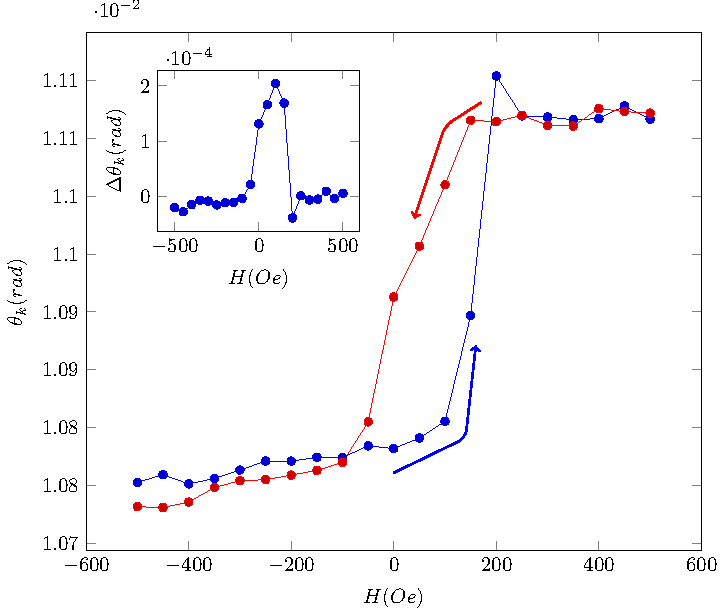
\includegraphics[scale=0.6]{resexp/his/HisTheta.pdf}
		\label{Exp:fig:theta}
	}
	\subfigure[Rotaci\'on Kerr]{
		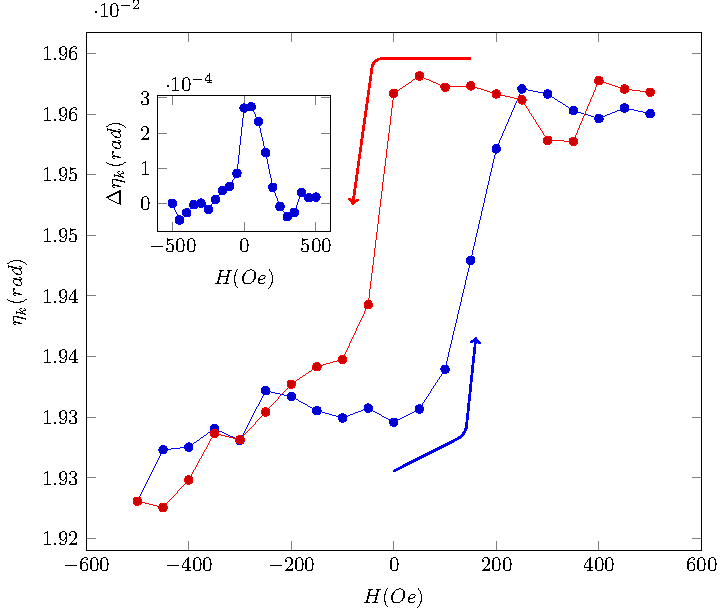
\includegraphics[scale=0.6]{resexp/his/HisEpsilon.pdf}
		\label{Exp:fig:elip}
	}
	\caption[Hit\'eresis de $\theta_k$ y $\eta_k$ en CoFeB]{Medici\'on de rotaci\'on (\ref{Exp:fig:theta}) y elipticidad (\ref{Exp:fig:elip}) Kerr en una muestra de CoFeB. Dentro de cada figura se muestra en cambio de la se\~nal medida con cada direcci\'on de campo magn\'etico.}
	\label{Exp:fig:Kerrhis}
	
\end{figure}
 \newline 
 \par A continuaci\'on se utiliz\'o la fuente supercontinua y se midieron espectros con y sin campo magn\'etico aplicado y se obtuvieron los resultados que se muestran en la figura \ref{Exp:fig:espectroK}. En dicha figura es posible observar un cambio en el \'angulo y elipticidad Kerr; adem\'as se muestran la forma de linea que se obtiene cuando la referencia de $2f$ del lock in con respecto al campo magn\'etico corresponden las energ\'ias del fot\'on de $1.42 ~eV~y~1.48~eV$; adem\'as se observan ciclos de hist\'eresis lo cual indica que se est\'a midiendo un efecto magneto-\'optico en el CoFeB. Se ha comparado esta se\~nal con espectros obtenidos con otras configuraciones y se ha encontrado similitud  \cite{Hoffmann_2019}.
\begin{figure}[!hbt]
	\centering
	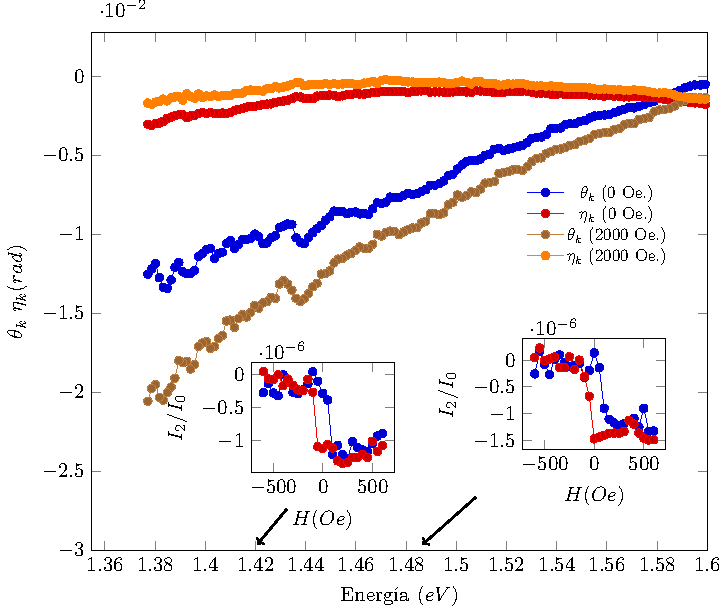
\includegraphics[scale=0.8]{resexp/esp/espectro0.pdf}
	\caption[Espectro de efecto Kerr magneto-\'optico]{Espectros del \'angulo y elipticidad Kerr en funci\'on de la energ\'ia del fot\'on en donde se induce un campo de $2000 Oe$.}
	\label{Exp:fig:espectroK}
\end{figure}
\section{Conclusiones}
Fu\'e posible  desarrollar un sistema de espectroscopia de Efecto Kerr magneto-\'optico partiendo de un montaje ya dise\~nado anteriormente y se desarroll\'o la instrumentaci\'on virtual para su control. Para asegurarnos  del correcto funcionamiento de este sistema se realizaron mediciones de hist\'eresis en una muestra de CoFeB y una vez que fu\'e posible obtenerlas, se procedi\'o a adquirir los valores de rotaci\'on y elipticidad en funci\'on de la longitud de onda. A partir  del an\'alisis de Jones fue posible notar que el separador de haz (beamsplitter) alteraba las mediciones y para poder realizar las correciones necesarias fue necesario medir elipsometr\'ia a 70 \degree a dicho beamsplitter y   se escribi\'o un c\'odigo en Python para poder adquirir la rotaci\'on ($\theta_k$) y la elipticidad ($\eta_k$)  Kerr tanto de las mediciones de hist\'eresis como del espectro a incidencia casi normal con el beamsplitter a 45 \degree.
    \bibliographystyle{ieeetr}
    \bibliography{refInt,ref,refKerr,refMet,refSim,refRel}
\end{document}

